%=============================================================================

共形场论（conformal field theory, CFT）是具有共形对称性的量子场论。共形对称性是比庞加莱对称性（Poincaré symmetry）更大的对称性群，它包含标度变换（scale transformation）和特殊共形变换（special conformal transformation）。在 AdS/CFT 对偶中，边界理论通常是一个共形场论 \cite{Maldacena1997}。共形对称性对关联函数施加了很强的约束，使得我们可以精确计算许多物理量 \cite{Aharony1999}。本节的内容为理解 AdS/CFT 对偶提供必要的基础。

\begin{note}[CFT 的物理应用]
CFT 在现代理论物理学中有着广泛的应用：
\begin{itemize}
    \item \textbf{临界现象}：连续相变的临界点处，关联长度发散，系统表现出尺度不变性，临界行为可以用 CFT 描述
    \item \textbf{弦理论}：弦的世界面理论是一个 2 维 CFT \cite{Polchinski1998}
    \item \textbf{凝聚态物理}：量子霍尔效应、自旋链、拓扑相变等都与 CFT 密切相关
    \item \textbf{AdS/CFT 对偶}：边界理论是一个 CFT，共形对称性是 AdS/CFT 的对称性基础 \cite{Maldacena1997}
\end{itemize}
\end{note}

%=============================================================================
\section{共形变换}

\begin{definition}[共形变换]
共形变换（conformal transformation）是保持角度不变的坐标变换。更精确地说，共形变换是保持度规形式不变，只改变其整体标度的变换：
\begin{equation}
    \bar{g}_{\mu\nu}(x') = \Omega^2(x) g_{\mu\nu}(x),
\end{equation}
其中 $\Omega(x) > 0$ 是标度因子（scale factor），它可以依赖于时空坐标。
\end{definition}

\begin{note}[直观理解]
想象一张橡皮膜，你可以在上面画图。共形变换就像是拉伸这张膜，但要求保持所有角度不变。这意味着你可以改变图形的大小，但不能改变它的形状。例如，一个正方形可以变成一个更大的正方形，但不能变成长方形。
\end{note}

\begin{remark}[因果结构]
共形变换保持两个曲线之间的角度不变，但可以改变长度的标度。这意味着共形变换保持因果结构（causal structure）不变，因为光锥（light cone）由角度定义。这是一个非常重要的物理性质：共形变换不改变物理系统的因果关系。
\end{remark}

\begin{theorem}[共形群与 AdS 等距群]
在 $d$ 维闵可夫斯基空间中，共形变换群是 $SO(2, d)$，这恰好等于 AdS$_{d+1}$ 空间的等距群（isometry group）。这是 AdS/CFT 对偶的对称性基础 \cite{Maldacena1997}。
\end{theorem}

\subsection{无穷小共形变换与共形 Killing 方程的推导}

\begin{note}[物理动机]
我们希望找到所有保持角度不变的无穷小坐标变换。这些变换构成了共形群，是 CFT 的对称性基础。在物理上，这意味着系统没有内在的特征长度尺度，这正是临界现象的特征。
\end{note}

\begin{theorem}[共形 Killing 方程的推导]
考虑无穷小坐标变换 $x^\mu \to x'^\mu = x^\mu + \epsilon^\mu(x)$。度规的变化为：
\begin{equation}
    g_{\mu\nu}(x) \to g'_{\mu\nu}(x') = g_{\mu\nu}(x) - \partial_\mu \epsilon_\nu - \partial_\nu \epsilon_\mu.
\end{equation}
共形变换要求度规只改变整体标度：
\begin{equation}
    g'_{\mu\nu}(x') = \Omega^2(x) g_{\mu\nu}(x) \approx (1 + 2\omega(x)) g_{\mu\nu}(x),
\end{equation}
其中 $\omega(x)$ 是无穷小标度因子。因此：
\begin{equation}
    \partial_\mu \epsilon_\nu + \partial_\nu \epsilon_\mu = 2\omega(x) \eta_{\mu\nu}.
    \label{eq:conformal_Killing_1}
\end{equation}
\end{theorem}

\begin{proof}[确定 $\omega(x)$ 的值]
对 \eqref{eq:conformal_Killing_1} 取迹（乘以 $\eta^{\mu\nu}$）：
\begin{equation}
    \eta^{\mu\nu} (\partial_\mu \epsilon_\nu + \partial_\nu \epsilon_\mu) = 2\omega(x) \eta^{\mu\nu} \eta_{\mu\nu} = 2\omega(x) d.
\end{equation}
左边为 $2\partial \cdot \epsilon$，因此：
\begin{equation}
    \omega(x) = \frac{1}{d} \partial \cdot \epsilon.
\end{equation}
代回 \eqref{eq:conformal_Killing_1}，得到\textbf{共形 Killing 方程}：
\begin{equation}
    \partial_\mu \epsilon_\nu + \partial_\nu \epsilon_\mu = \frac{2}{d} (\partial \cdot \epsilon) \eta_{\mu\nu}.
    \label{eq:conformal_Killing}
\end{equation}
满足这个方程的矢量场 $\epsilon^\mu$ 称为\textbf{共形 Killing 矢量}（conformal Killing vector）。
\end{proof}

\begin{remark}
共形 Killing 方程 \eqref{eq:conformal_Killing} 的物理意义是：无穷小坐标变换保持角度不变，当且仅当度规的变化是整体标度变换。这比一般的等距变换（保持度规不变）更宽松，因此共形群比等距群更大。
\end{remark}

\begin{figure}[htbp]
\centering
\begin{tikzpicture}[scale=1.0]
    % 平移
    \draw[thick, blue, ->] (0,0) -- (1.5,0) node[midway, below] {$a^\mu$};
    \draw[thick, blue] (0,0) rectangle (1,1);
    \draw[thick, blue, dashed] (1.5,0) rectangle (2.5,1);
    \node at (0.5, 1.3) {\small 原始图形};
    \node at (2.0, 1.3) {\small 平移};
    % 旋转
    \draw[thick, red] (4,0) rectangle (5,1);
    \draw[thick, red, dashed, rotate=30] (4,0) rectangle (5,1);
    \node at (4.5, 1.3) {\small 旋转};
    % 标度
    \draw[thick, green!60!black] (7,0) rectangle (8,1);
    \draw[thick, green!60!black, dashed] (7,0) rectangle (8.5,1.5);
    \node at (7.5, 1.8) {\small 标度变换};
\end{tikzpicture}
\caption{共形变换的直观理解：平移保持图形不变，旋转保持角度和距离不变，标度变换改变大小但保持角度不变。}
\label{fig:conformal_transformations}
\end{figure}

\subsection{共形 Killing 方程的解}

\begin{theorem}[共形 Killing 方程的一般解]
共形 Killing 方程 \eqref{eq:conformal_Killing} 的一般解为：
\begin{equation}
    \epsilon^\mu(x) = a^\mu + {\omega^\mu}_\nu x^\nu + \lambda x^\mu + (b \cdot x) x^\mu - \frac{1}{2} b^\mu x^2,
\end{equation}
其中：
\begin{itemize}
    \item $a^\mu$：平移参数（$d$ 个）
    \item $\omega_{\mu\nu} = -\omega_{\nu\mu}$：旋转参数（$d(d-1)/2$ 个）
    \item $\lambda$：标度变换参数（1 个）
    \item $b^\mu$：特殊共形变换参数（$d$ 个）
\end{itemize}
\end{theorem}

\begin{proof}[参数计数]
总参数数目为 $d + d(d-1)/2 + 1 + d = d(d+3)/2 + 1$。去掉整体标度（它不改变物理），独立参数数目为 $d(d+3)/2$，这正是共形群 $SO(2,d)$ 的维数：
\begin{equation}
    \dim SO(2,d) = \frac{(d+2)(d+1)}{2} - 1 = \frac{d(d+3)}{2}.
\end{equation}
对于 $d=4$，共形群有 15 个生成元。这比庞加莱群的 10 个生成元多出 5 个，多出的就是标度变换和 4 个特殊共形变换。
\end{proof}

\begin{example}[各变换的物理意义]
\begin{itemize}
    \item $a^\mu$：将整个系统平移 $a^\mu$，不改变任何物理性质
    \item $\omega_{\mu\nu}$：将系统旋转，保持距离不变
    \item $\lambda$：将系统整体放大或缩小，但保持形状不变
    \item $b^\mu$：特殊共形变换，可以理解为先做反演变换，然后平移，然后再做反演变换
\end{itemize}
\end{example}

\subsection{有限共形变换}

从无穷小变换可以积分得到有限变换。四种基本的有限共形变换为：

\begin{definition}[平移]
\begin{equation}
    x'^\mu = x^\mu + a^\mu.
\end{equation}
\end{definition}

\begin{definition}[旋转]
\begin{equation}
    x'^\mu = {\Lambda^\mu}_\nu x^\nu, \quad \Lambda^T \eta \Lambda = \eta.
\end{equation}
\end{definition}

\begin{definition}[标度变换]
\begin{equation}
    x'^\mu = \lambda x^\mu, \quad \lambda > 0.
\end{equation}
标度变换将所有长度缩放 $\lambda$ 倍，但保持角度不变。
\end{definition}

\begin{definition}[特殊共形变换]
\begin{equation}
    x'^\mu = \frac{x^\mu - b^\mu x^2}{1 - 2b \cdot x + b^2 x^2}.
\end{equation}
\end{definition}

\begin{proof}[特殊共形变换的分解]
特殊共形变换可以分解为三步：
\begin{enumerate}
    \item 反演变换 $x^\mu \to x^\mu/x^2$
    \item 平移 $x^\mu \to x^\mu - b^\mu$
    \item 再次反演变换 $x^\mu \to x^\mu/x^2$
\end{enumerate}
验证：设 $I(x^\mu) = x^\mu/x^2$，则 $I(I(x^\mu)) = x^\mu$。组合 $I \circ T_{-b} \circ I$ 给出：
\begin{equation}
    x^\mu \xrightarrow{I} \frac{x^\mu}{x^2} \xrightarrow{T_{-b}} \frac{x^\mu}{x^2} - b^\mu \xrightarrow{I} \frac{x^\mu - b^\mu x^2}{|x - b x^2|^2} = \frac{x^\mu - b^\mu x^2}{1 - 2b \cdot x + b^2 x^2}.
\end{equation}
\end{proof}

\subsection{反演变换与物理意义}

\begin{definition}[反演变换]
反演变换（inversion）是特殊共形变换的基本组成部分：
\begin{equation}
    x^\mu \to \frac{x^\mu}{x^2}.
\end{equation}
反演变换将靠近原点的点映射到远离原点的点，反之亦然。在反演变换下，度规变换为：
\begin{equation}
    g_{\mu\nu} \to \frac{1}{(x^2)^2} g_{\mu\nu}.
\end{equation}
因此反演变换是共形变换，标度因子为 $\Omega(x) = 1/x^2$。
\end{definition}

\begin{remark}[共形不变性与标度不变性]
共形不变性是比标度不变性更强的对称性。标度不变性只要求系统在整体缩放下不变，而共形不变性还要求在特殊共形变换下不变。在大多数情况下，标度不变性自动蕴含共形不变性，但也存在反例。
\end{remark}

%=============================================================================
\section{共形代数}

\begin{definition}[共形变换的生成元]
共形变换的生成元（generators of conformal transformations）为：
\begin{itemize}
    \item \textbf{平移}：$P_\mu = -i\partial_\mu$。平移生成元将系统在时空中整体移动，不改变系统的任何内部性质。
    \item \textbf{旋转}：$M_{\mu\nu} = i(x_\mu \partial_\nu - x_\nu \partial_\mu)$。旋转生成元将系统绕某个轴旋转，保持系统的距离不变。
    \item \textbf{标度变换}：$D = -ix^\mu \partial_\mu$。标度变换将系统整体放大或缩小，但保持形状不变。这是共形对称性特有的生成元。
    \item \textbf{特殊共形变换}：$K_\mu = i(x^2 \partial_\mu - 2x_\mu x^\nu \partial_\nu)$。特殊共形变换是一种更复杂的变换，它可以被理解为先做反演变换（inversion），然后平移，然后再做反演变换。
\end{itemize}
\end{definition}

\begin{theorem}[共形代数]
这些生成元满足李代数（Lie algebra）：
\begin{align}
    [D, P_\mu] &= iP_\mu, \label{eq:conf_alg_1}\\
    [D, K_\mu] &= -iK_\mu, \label{eq:conf_alg_2}\\
    [K_\mu, P_\nu] &= 2i(\eta_{\mu\nu}D - M_{\mu\nu}), \label{eq:conf_alg_3}\\
    [M_{\mu\nu}, P_\rho] &= i(\eta_{\nu\rho}P_\mu - \eta_{\mu\rho}P_\nu), \label{eq:conf_alg_4}\\
    [M_{\mu\nu}, K_\rho] &= i(\eta_{\nu\rho}K_\mu - \eta_{\mu\rho}K_\nu), \label{eq:conf_alg_5}\\
    [M_{\mu\nu}, M_{\rho\sigma}] &= i(\eta_{\nu\rho}M_{\mu\sigma} - \eta_{\mu\rho}M_{\nu\sigma} - \eta_{\nu\sigma}M_{\mu\rho} + \eta_{\mu\sigma}M_{\nu\rho}). \label{eq:conf_alg_6}
\end{align}
\end{theorem}

\begin{proof}[对易关系 $[D, P_\mu] = iP_\mu$ 的推导]
将生成元作用于测试函数 $f(x)$：
\begin{align}
    [D, P_\mu] f(x) &= (-ix^\nu \partial_\nu)(-i\partial_\mu) f - (-i\partial_\mu)(-ix^\nu \partial_\nu) f \notag \\
    &= -x^\nu \partial_\nu \partial_\mu f + \partial_\mu (x^\nu \partial_\nu f) \notag \\
    &= -x^\nu \partial_\nu \partial_\mu f + \delta_\mu^\nu \partial_\nu f + x^\nu \partial_\mu \partial_\nu f \notag \\
    &= \partial_\mu f = iP_\mu f.
\end{align}
因此 $[D, P_\mu] = iP_\mu$。
\end{proof}

\begin{proof}[对易关系 $[K_\mu, P_\nu]$ 的推导]
计算 $[K_\mu, P_\nu]$ 作用于 $f(x)$：
\begin{align}
    [K_\mu, P_\nu] f &= i(x^2 \partial_\mu - 2x_\mu x^\rho \partial_\rho)(-i\partial_\nu) f - (-i\partial_\nu) i(x^2 \partial_\mu - 2x_\mu x^\rho \partial_\rho) f \notag \\
    &= (x^2 \partial_\mu - 2x_\mu x^\rho \partial_\rho)\partial_\nu f - \partial_\nu(x^2 \partial_\mu f - 2x_\mu x^\rho \partial_\rho f).
\end{align}
展开第二项：
\begin{align}
    \partial_\nu(x^2 \partial_\mu f) &= 2x_\nu \partial_\mu f + x^2 \partial_\nu \partial_\mu f, \\
    \partial_\nu(2x_\mu x^\rho \partial_\rho f) &= 2\eta_{\mu\nu} x^\rho \partial_\rho f + 2x_\mu \partial_\nu f + 2x_\mu x^\rho \partial_\rho \partial_\nu f.
\end{align}
合并后得到：
\begin{equation}
    [K_\mu, P_\nu] f = -2x_\nu \partial_\mu f + 2\eta_{\mu\nu} x^\rho \partial_\rho f - 2x_\mu \partial_\nu f.
\end{equation}
注意到 $2\eta_{\mu\nu} x^\rho \partial_\rho f = -2i\eta_{\mu\nu} D f$，而 $-2(x_\nu \partial_\mu - x_\mu \partial_\nu) f = -2i M_{\mu\nu} f$，因此：
\begin{equation}
    [K_\mu, P_\nu] = 2i(\eta_{\mu\nu} D - M_{\mu\nu}).
\end{equation}
\end{proof}

\begin{note}[对易关系的物理意义]
这些对易关系告诉我们，标度变换 $D$ 可以将平移生成元 $P_\mu$ "放大"或"缩小"。这意味着在标度变换下，动量的量纲会发生变化。这正是共形维数的物理来源。
\end{note}

\subsection{共形代数的结构}

\begin{theorem}[$SO(2,d)$ 的实现]
共形代数 \eqref{eq:conf_alg_1}-\eqref{eq:conf_alg_6} 可以用更统一的方式理解。定义：
\begin{equation}
    J_{AB} = \{M_{\mu\nu}, P_\mu, K_\mu, D\}, \quad A, B = -1, 0, 1, \ldots, d,
\end{equation}
则共形代数可以写成：
\begin{equation}
    [J_{AB}, J_{CD}] = i(\eta_{AD}J_{BC} - \eta_{AC}J_{BD} + \eta_{BC}J_{AD} - \eta_{BD}J_{AC}),
\end{equation}
其中 $\eta_{AB} = \text{diag}(-1,-1,+1,\ldots,+1)$。这正是 $SO(2,d)$ 的李代数。
\end{theorem}

\begin{property}[生成元的对应关系]
\begin{align}
    M_{\mu\nu} &= J_{\mu\nu}, & P_\mu &= J_{-1,\mu} + J_{0,\mu}, \notag \\
    K_\mu &= J_{-1,\mu} - J_{0,\mu}, & D &= J_{-1,0}.
\end{align}
\end{property}

\subsection{与 AdS 等距群的对应}

\begin{theorem}[共形代数与 AdS 等距代数的同构]
共形代数与 AdS$_{d+1}$ 的等距代数完全相同。这个对应关系是 AdS/CFT 对偶的对称性基础 \cite{Maldacena1997}：
\begin{center}
\begin{tabular}{|c|c|}
\hline
\textbf{CFT 共形变换} & \textbf{AdS 等距变换} \\
\hline
平移 $P_\mu$ & AdS 中的平移 \\
旋转 $M_{\mu\nu}$ & AdS 中的旋转 \\
标度变换 $D$ & AdS 中的径向平移 \\
特殊共形变换 $K_\mu$ & AdS 中的特殊等距 \\
\hline
\end{tabular}
\end{center}
\end{theorem}

%=============================================================================
\section{共形维数和初级算符}

\begin{definition}[共形维数]
在标度变换 $x \to \lambda x$ 下，算符 $\mathcal{O}(x)$ 的变换规律为：
\begin{equation}
    \mathcal{O}(x) \to \lambda^{-\Delta} \mathcal{O}(\lambda x),
\end{equation}
其中 $\Delta$ 称为共形维数（conformal dimension）。共形维数度量算符在标度变换下的"权重"：当我们将系统放大 $\lambda$ 倍时，算符的值会乘以 $\lambda^{-\Delta}$。
\end{definition}

\subsection{初级算符的定义}

\begin{definition}[初级算符]
初级算符（primary operator）是共形群的"最低权态"，它满足：
\begin{equation}
    [K_\mu, \mathcal{O}(x)] = 0, \quad [D, \mathcal{O}(x)] = -i\Delta \mathcal{O}(x).
\end{equation}
\end{definition}

\begin{note}[物理动机]
在量子场论中，所有其他态都可以通过对基本粒子作用动量算符得到。类似地，在 CFT 中，所有其他算符都可以通过对初级算符作用平移生成元 $P_\mu$ 得到。这些通过对初级算符作用平移生成元得到的算符称为后裔算符（descendant operator），例如 $\partial_\mu \mathcal{O}(x)$ 是 $\mathcal{O}(x)$ 的后裔算符。
\end{note}

\subsection{初级算符的变换规律}

在一般的共形变换下，初级算符的变换规律为：

\begin{property}[平移变换]
\begin{equation}
    e^{ia^\mu P_\mu} \mathcal{O}(x) e^{-ia^\mu P_\mu} = \mathcal{O}(x+a).
\end{equation}
\end{property}

\begin{property}[标度变换]
\begin{equation}
    e^{i\lambda D} \mathcal{O}(x) e^{-i\lambda D} = e^{-\lambda \Delta} \mathcal{O}(e^\lambda x).
\end{equation}
\end{property}

\begin{property}[旋转变换]
\begin{equation}
    e^{i\frac{1}{2}\omega^{\mu\nu}M_{\mu\nu}} \mathcal{O}(x) e^{-i\frac{1}{2}\omega^{\mu\nu}M_{\mu\nu}} = {R^{-1}}^\Delta_\Delta \mathcal{O}(R x),
\end{equation}
其中 $R$ 是旋转矩阵，对于标量算符 ${R^{-1}}^\Delta_\Delta = 1$。
\end{property}

\begin{property}[特殊共形变换]
\begin{equation}
    e^{ib^\mu K_\mu} \mathcal{O}(x) e^{-ib^\mu K_\mu} = |1 - 2b \cdot x + b^2 x^2|^\Delta \mathcal{O}\left(\frac{x - b x^2}{1 - 2b \cdot x + b^2 x^2}\right).
\end{equation}
\end{property}

\subsection{不同场的共形维数}

\begin{note}[物理动机]
在 CFT 中，不同类型的场具有不同的共形维数。这些共形维数可以通过对称性分析来确定。共形维数与场的质量量纲密切相关，在 AdS/CFT 对偶中，它与体空间中对应场的质量直接相关。
\end{note}

\begin{property}[基本场的共形维数]
在 $d$ 维 CFT 中，基本场的共形维数为：
\begin{itemize}
    \item \textbf{标量场} $\phi(x)$：$\Delta = (d-2)/2$
    \item \textbf{费米子场} $\psi(x)$：$\Delta = (d-1)/2$
    \item \textbf{守恒流} $J_\mu(x)$：$\Delta = d-1$
    \item \textbf{应力张量} $T_{\mu\nu}(x)$：$\Delta = d$
\end{itemize}
\end{property}

\begin{example}[4 维 CFT 中的共形维数]
在 4 维 CFT 中（$d=4$）：
\begin{itemize}
    \item 标量场：$\Delta = 1$，这意味着标量场在标度变换下像长度的倒数一样变换
    \item 费米子场：$\Delta = 3/2$，费米子场的共形维数比标量场大，这意味着费米子场在短距离下衰减得更快
    \item 守恒流：$\Delta = 3$，守恒流的共形维数与其守恒律密切相关
    \item 应力张量：$\Delta = 4$，应力张量是 CFT 中最重要的算符之一，因为它与能量-动量守恒相关
\end{itemize}
\end{example}

\begin{note}[共形维数的物理意义]
共形维数 $\Delta$ 度量了算符在标度变换下的"权重"：
\begin{itemize}
    \item 当我们将系统放大 $\lambda$ 倍时，算符的值会乘以 $\lambda^{-\Delta}$
    \item 这类似于物理学中的量纲分析：能量的量纲是 1，长度的量纲是 -1
    \item 在 AdS/CFT 对偶中，共形维数与体空间中对应场的质量相关：$\Delta(\Delta-d) = m^2 L^2$ \cite{Gubser1998}
\end{itemize}
\end{note}

\subsection{共形维数与自旋}

\begin{definition}[幺正性界]
对于具有自旋的算符，共形维数和自旋共同确定了算符在共形变换下的行为。在 $d$ 维空间中，算符由两个量子数标记：共形维数 $\Delta$ 和自旋 $l$（或更一般地，由 $SO(d)$ 的表示标记）。

对于标量算符（$l = 0$），共形维数满足幺正性界：
\begin{equation}
    \Delta \geq \frac{d-2}{2}.
\end{equation}
对于守恒流（$l = 1$），$\Delta = d-1$。对于应力张量（$l = 2$），$\Delta = d$。
\end{definition}

\begin{remark}
当幺正性界的等号成立时，对应的算符是守恒的。例如，$\Delta = d-1$ 对应守恒流，$\Delta = d$ 对应守恒应力张量。这些守恒算符在 AdS/CFT 对偶中对应于规范场和引力场 \cite{Witten1998}。
\end{remark}

\subsection{后裔算符}

\begin{definition}[后裔算符]
后裔算符是通过对初级算符作用平移生成元得到的算符。对于标量初级算符 $\mathcal{O}(x)$，后裔算符为：
\begin{align}
    \text{一级后裔：} & \quad \partial_\mu \mathcal{O}(x), \quad \Delta_{\text{desc}} = \Delta + 1, \notag \\
    \text{二级后裔：} & \quad \partial_\mu \partial_\nu \mathcal{O}(x), \quad \Delta_{\text{desc}} = \Delta + 2, \notag \\
    \text{一般后裔：} & \quad \partial_{\mu_1} \cdots \partial_{\mu_n} \mathcal{O}(x), \quad \Delta_{\text{desc}} = \Delta + n.
\end{align}
\end{definition}

\begin{remark}
后裔算符不是独立的算符——它们可以通过初级算符和共形代数来表示。在 CFT 的希尔伯特空间中，后裔算符构成"共形家族"的一部分。
\end{remark}

%=============================================================================
\section{共形对称性对关联函数的约束}

共形对称性对关联函数施加很强的约束，使得我们可以精确确定低点关联函数的形式。这是 CFT 最强大的性质之一：即使我们不知道理论的详细动力学，共形对称性也能告诉我们很多信息。

\subsection{一点函数的约束}

\begin{theorem}[一点函数为零]
对于非平庸的初级算符，一点函数必须为零：
\begin{equation}
    \langle \mathcal{O}(x) \rangle = 0.
\end{equation}
\end{theorem}

\begin{proof}
在标度变换下，一点函数变换为：
\begin{equation}
    \langle \mathcal{O}(x) \rangle \to \lambda^{-\Delta} \langle \mathcal{O}(\lambda x) \rangle.
\end{equation}
如果 $\langle \mathcal{O}(x) \rangle = c \neq 0$（常数），则 $c = \lambda^{-\Delta} c$，这对 $\Delta \neq 0$ 矛盾。因此 $c = 0$。
\end{proof}

\begin{remark}
对于恒等算符 $\mathbf{1}$（$\Delta = 0$），一点函数 $\langle \mathbf{1} \rangle = 1$ 是非零的。这是唯一一个具有非零一点函数的初级算符。
\end{remark}

\subsection{两点函数的详细推导}

\begin{note}[物理动机]
在 CFT 中，两点函数 $\langle \mathcal{O}(x) \mathcal{O}(y) \rangle$ 描述了两个算符之间的关联。由于 CFT 没有特征长度尺度，关联函数只能以幂律形式衰减，而不是指数形式（指数衰减对应于有质量粒子，而 CFT 中的粒子是无质量的）。
\end{note}

\begin{theorem}[两点函数的形式]
共形对称性完全确定两点函数的形式（除了归一化常数）：
\begin{equation}
    \langle \mathcal{O}_1(x) \mathcal{O}_2(y) \rangle = \frac{C_{\mathcal{O}_1\mathcal{O}_2} \delta_{\Delta_1, \Delta_2}}{|x - y|^{2\Delta}}.
\end{equation}
\end{theorem}

\begin{proof}[详细推导]
考虑两点函数 $\langle \mathcal{O}_1(x) \mathcal{O}_2(y) \rangle$。我们要求这个函数在所有共形变换下不变。

\textbf{步骤 1：平移不变性}。在平移变换 $x \to x + a$，$y \to y + a$ 下，两点函数不变：
\begin{equation}
    \langle \mathcal{O}_1(x) \mathcal{O}_2(y) \rangle = \langle \mathcal{O}_1(x+a) \mathcal{O}_2(y+a) \rangle.
\end{equation}
这意味着两点函数只能依赖于坐标差 $x - y$：
\begin{equation}
    \langle \mathcal{O}_1(x) \mathcal{O}_2(y) \rangle = f(x - y).
\end{equation}

\textbf{步骤 2：旋转不变性}。在旋转变换 $x \to Rx$，$y \to Ry$ 下，两点函数不变：
\begin{equation}
    \langle \mathcal{O}_1(x) \mathcal{O}_2(y) \rangle = \langle \mathcal{O}_1(Rx) \mathcal{O}_2(Ry) \rangle.
\end{equation}
这意味着 $f(x - y)$ 只能依赖于 $|x - y|$（旋转不变量）：
\begin{equation}
    \langle \mathcal{O}_1(x) \mathcal{O}_2(y) \rangle = g(|x - y|).
\end{equation}

\textbf{步骤 3：标度不变性}。在标度变换 $x \to \lambda x$，$y \to \lambda y$ 下：
\begin{equation}
    \langle \mathcal{O}_1(x) \mathcal{O}_2(y) \rangle = \lambda^{-\Delta_1 - \Delta_2} \langle \mathcal{O}_1(\lambda x) \mathcal{O}_2(\lambda y) \rangle.
\end{equation}
这意味着：
\begin{equation}
    g(|x - y|) = \lambda^{-\Delta_1 - \Delta_2} g(\lambda |x - y|).
\end{equation}
令 $r = |x-y|$，上式对任意 $\lambda$ 成立。令 $\lambda = 1/r$，得 $g(r) = r^{\Delta_1+\Delta_2} g(1)$，即：
\begin{equation}
    g(r) = \frac{C}{r^{\Delta_1 + \Delta_2}}.
\end{equation}

\textbf{步骤 4：算符的归一化}。对于相同的算符 $\mathcal{O}_1 = \mathcal{O}_2 = \mathcal{O}$，$\Delta_1 = \Delta_2 = \Delta$：
\begin{equation}
    \langle \mathcal{O}(x) \mathcal{O}(y) \rangle = \frac{C_{\mathcal{O}\mathcal{O}}}{|x - y|^{2\Delta}}.
\end{equation}
\end{proof}

\begin{figure}[htbp]
\centering
\begin{tikzpicture}[scale=1.2]
    % 绘制坐标轴
    \draw[thick, ->] (0,0) -- (5,0) node[right] {$|x - y|$};
    \draw[thick, ->] (0,0) -- (0,4) node[above] {$\langle \mathcal{O}(x) \mathcal{O}(y) \rangle$};
    
    % 绘制两点函数
    \draw[thick, blue, domain=0.5:4.5, samples=100] 
        plot (\x, {3/\x^2});
    
    % 标注幂律行为
    \node at (3,3) {$\sim 1/|x-y|^{2\Delta}$};
    
    % 标注共形维数
    \draw[dashed, red] (0,0) -- (4,2) node[midway, above left] {$\Delta$ 越大，衰减越快};
\end{tikzpicture}
\caption{CFT 中两点函数的幂律行为。关联函数以幂律形式衰减，衰减的快慢由共形维数 $\Delta$ 决定。}
\label{fig:two_point}
\end{figure}

\begin{note}[两点函数的物理意义]
两点函数的幂律形式 $\sim 1/|x-y|^{2\Delta}$ 反映了 CFT 中没有特征长度尺度：
\begin{itemize}
    \item \textbf{无特征长度}：CFT 中没有内在的长度尺度，所有长度都是等价的。这导致关联函数以幂律形式衰减，而不是指数形式。
    \item \textbf{共形维数}：$\Delta$ 越大，衰减越快。这意味着高维算符在短距离下衰减得更快。
    \item \textbf{正交性}：两点函数只在两个算符具有相同共形维数时才不为零。这意味着在 CFT 中，不同共形维数的算符是"正交"的。
\end{itemize}
\end{note}

\subsection{三点函数的详细推导}

\begin{note}[物理动机]
三点函数描述了三个算符之间的关联。在微扰理论中，三点函数对应于相互作用顶点。在 CFT 中，三点函数完全由共形对称性确定，唯一的自由度是 OPE 系数 $C_{123}$，它包含了理论的非平庸信息。
\end{note}

\begin{theorem}[三点函数的形式]
共形对称性完全确定三点函数的形式（除了 OPE 系数）：
\begin{equation}
    \langle \mathcal{O}_1(x) \mathcal{O}_2(y) \mathcal{O}_3(z) \rangle = \frac{C_{123}}{|x - y|^{\Delta_1 + \Delta_2 - \Delta_3} |y - z|^{\Delta_2 + \Delta_3 - \Delta_1} |x - z|^{\Delta_3 + \Delta_1 - \Delta_2}}.
\end{equation}
\end{theorem}

\begin{proof}[详细推导]
考虑三点函数 $\langle \mathcal{O}_1(x) \mathcal{O}_2(y) \mathcal{O}_3(z) \rangle$。

\textbf{步骤 1：平移不变性}。三点函数只能依赖于坐标差：
\begin{equation}
    \langle \mathcal{O}_1(x) \mathcal{O}_2(y) \mathcal{O}_3(z) \rangle = f(x - y, y - z).
\end{equation}

\textbf{步骤 2：旋转不变性}。$f$ 只能依赖于旋转不变量：
\begin{equation}
    |x - y|, \quad |y - z|, \quad |x - z|.
\end{equation}

\textbf{步骤 3：标度不变性}。在标度变换下：
\begin{equation}
    \langle \mathcal{O}_1(x) \mathcal{O}_2(y) \mathcal{O}_3(z) \rangle = \lambda^{-\Delta_1 - \Delta_2 - \Delta_3} \langle \mathcal{O}_1(\lambda x) \mathcal{O}_2(\lambda y) \mathcal{O}_3(\lambda z) \rangle.
\end{equation}
这意味着 $f$ 必须具有以下形式：
\begin{equation}
    f = \frac{h(\text{角度})}{|x - y|^{\alpha} |y - z|^{\beta} |x - z|^{\gamma}},
\end{equation}
其中 $\alpha + \beta + \gamma = \Delta_1 + \Delta_2 + \Delta_3$。

\textbf{步骤 4：特殊共形不变性}。特殊共形变换对三点函数施加了更强的约束。通过要求三点函数在特殊共形变换下不变，可以唯一地确定各幂次：
\begin{align}
    \alpha &= \Delta_1 + \Delta_2 - \Delta_3, \\
    \beta &= \Delta_2 + \Delta_3 - \Delta_1, \\
    \gamma &= \Delta_3 + \Delta_1 - \Delta_2.
\end{align}
\end{proof}

\begin{remark}
三点函数的形式完全由共形对称性确定，唯一的自由度是 OPE 系数 $C_{123}$。这意味着，如果我们知道所有 OPE 系数，我们就完全知道了 CFT。OPE 系数是 CFT 的"耦合常数"，它们决定了不同算符之间的相互作用强度。
\end{remark}

\subsection{四点函数与共形块}

\begin{definition}[共形不变量]
共形对称性不能完全确定四点函数及更高点函数的形式，但可以将其写成共形块（conformal block）的展开。定义共形不变量（conformal cross-ratios）：
\begin{equation}
    u = \frac{x_{12}^2 x_{34}^2}{x_{13}^2 x_{24}^2}, \quad v = \frac{x_{14}^2 x_{23}^2}{x_{13}^2 x_{24}^2}.
\end{equation}
共形不变量 $u$ 和 $v$ 在共形变换下保持不变，它们完全确定了四个点的"形状"，与它们的绝对位置和大小无关。
\end{definition}

\begin{theorem}[共形块展开]
四点函数可以展开为：
\begin{equation}
    \langle \mathcal{O}_1(x_1) \mathcal{O}_2(x_2) \mathcal{O}_3(x_3) \mathcal{O}_4(x_4) \rangle = \sum_{\mathcal{O}} C_{12\mathcal{O}} C_{34\mathcal{O}} G_{\Delta, l}(u, v),
\end{equation}
其中 $G_{\Delta, l}(u, v)$ 是共形块 \cite{Aharony1999}。
\end{theorem}

\begin{note}[物理解释]
共形块展开类似于量子力学中的分波展开（partial wave expansion）。在散射理论中，我们可以将散射振幅展开为不同角动量的贡献之和。类似地，在 CFT 中，我们可以将四点函数展开为不同"共形自旋"的贡献之和。
\end{note}

\begin{remark}
四点函数包含了 CFT 的完整动力学信息。OPE 系数 $C_{ij}^k$ 和共形维数 $\Delta_k$ 完全确定了四点函数，因此也完全确定了 CFT。这些数据称为 CFT 的\textbf{共形数据}（conformal data）。
\end{remark}

%=============================================================================
\section{共形 Ward 恒等式}

共形对称性导致了关联函数满足一系列约束条件，称为共形 Ward 恒等式。这些恒等式将守恒律与关联函数的对称性联系起来。

\begin{theorem}[平移 Ward 恒等式]
平移不变性要求：
\begin{equation}
    \sum_{i=1}^n \frac{\partial}{\partial x_i^\mu} \langle \mathcal{O}_1(x_1) \cdots \mathcal{O}_n(x_n) \rangle = 0.
\end{equation}
这意味着关联函数只能依赖于坐标差 $x_i - x_j$。
\end{theorem}

\begin{theorem}[旋转 Ward 恒等式]
旋转不变性要求：
\begin{equation}
    \sum_{i=1}^n \left( x_i^\mu \frac{\partial}{\partial x_i^\nu} - x_i^\nu \frac{\partial}{\partial x_i^\mu} \right) \langle \mathcal{O}_1(x_1) \cdots \mathcal{O}_n(x_n) \rangle = \text{自旋贡献}.
\end{equation}
\end{theorem}

\begin{theorem}[标度 Ward 恒等式]
标度不变性要求：
\begin{equation}
    \sum_{i=1}^n \left( x_i^\mu \frac{\partial}{\partial x_i^\mu} + \Delta_i \right) \langle \mathcal{O}_1(x_1) \cdots \mathcal{O}_n(x_n) \rangle = 0.
\end{equation}
这个方程表明，关联函数的标度维数必须等于各算符共形维数之和。
\end{theorem}

\begin{theorem}[特殊共形 Ward 恒等式]
特殊共形不变性要求：
\begin{equation}
    \sum_{i=1}^n \left( 2x_i^\mu (x_i \cdot \partial_i) - x_i^2 \partial_i^\mu + 2\Delta_i x_i^\mu \right) \langle \mathcal{O}_1(x_1) \cdots \mathcal{O}_n(x_n) \rangle = 0.
\end{equation}
这个方程是最强的约束，它将关联函数的形式几乎完全固定。
\end{theorem}

\begin{example}[两点函数的 Ward 恒等式验证]
对于两点函数 $\langle \mathcal{O}(x) \mathcal{O}(y) \rangle = C/|x-y|^{2\Delta}$，验证标度 Ward 恒等式：
\begin{equation}
    \left( x^\mu \partial_\mu + y^\mu \partial_\mu + 2\Delta \right) \frac{C}{|x-y|^{2\Delta}}.
\end{equation}
由于 $|x-y|^{2\Delta}$ 在标度变换 $x \to \lambda x$, $y \to \lambda y$ 下获得因子 $\lambda^{2\Delta}$，而算符获得因子 $\lambda^{-2\Delta}$，总效果为零。
\end{example}

%=============================================================================
\section{共形代数和表示理论}

共形群的表示理论是理解 CFT 的基础，它告诉我们 CFT 的希尔伯特空间是如何组织的。

在 $d$ 维欧几里得空间中，共形代数同构于 $SO(d+1,1)$ 的李代数。在 $d$ 维闵可夫斯基空间中，共形代数同构于 $SO(2,d)$ 的李代数。

\begin{definition}[共形家族]
CFT 的希尔伯特空间可以分解为共形群的最高权表示（highest weight representation）。每个最高权表示由一个初级算符 $\mathcal{O}$ 标记，包含该初级算符及其所有后裔算符。最高权表示可以理解为"粒子多重态"：在粒子物理学中，一个粒子多重态包含具有不同自旋投影的粒子；类似地，在 CFT 中，一个共形家族（conformal family）包含具有不同导数的算符。
\end{definition}

\begin{example}[标量初级算符的共形家族]
考虑一个标量初级算符 $\mathcal{O}(x)$，其共形维数为 $\Delta$。它的共形家族包含：
\begin{itemize}
    \item 初级算符：$\mathcal{O}(x)$，共形维数 $\Delta$
    \item 一级后裔：$\partial_\mu \mathcal{O}(x)$，共形维数 $\Delta + 1$
    \item 二级后裔：$\partial_\mu \partial_\nu \mathcal{O}(x)$，共形维数 $\Delta + 2$
    \item 以此类推...
\end{itemize}
\end{example}

\begin{figure}[htbp]
\centering
\begin{tikzpicture}[scale=0.9]
    % 算符-态对应
    \node[draw, circle, fill=blue!20] (vac) at (0,0) {$|0\rangle$};
    \node[draw, circle, fill=red!20] (O) at (3,0) {$\mathcal{O}(0)|0\rangle$};
    \node[draw, circle, fill=green!20] (PO1) at (6,0.5) {$P_\mu \mathcal{O}(0)|0\rangle$};
    \node[draw, circle, fill=green!20] (PO2) at (6,-0.5) {$P_\nu \mathcal{O}(0)|0\rangle$};
    \node[draw, circle, fill=yellow!20] (PPO) at (9,0) {$P_\mu P_\nu \mathcal{O}(0)|0\rangle$};
    \draw[thick, ->] (O) -- (PO1) node[midway, above left] {$P_\mu$};
    \draw[thick, ->] (O) -- (PO2) node[midway, below left] {$P_\nu$};
    \draw[thick, ->] (PO1) -- (PPO);
    \draw[thick, ->] (PO2) -- (PPO);
    \node at (3, -1.5) {\small 初级算符 $\Delta$};
    \node at (6, 1.5) {\small 一级后裔 $\Delta+1$};
    \node at (9, 1.0) {\small 二级后裔 $\Delta+2$};
\end{tikzpicture}
\caption{状态-算符对应与共形家族。初级算符 $\mathcal{O}(0)$ 作用于真空态产生初级态，后裔态通过对初级态作用平移生成元 $P_\mu$ 得到。}
\label{fig:state_operator}
\end{figure}

\subsection{幺正性界}

\begin{theorem}[幺正性界]
CFT 的表示理论对共形维数施加了重要的约束。对于幺正的 CFT，初级算符的共形维数必须满足：
\begin{align}
    \text{标量算符：} & \quad \Delta \geq \frac{d-2}{2}, \\
    \text{自旋 } l \text{ 算符：} & \quad \Delta \geq d - 2 + l.
\end{align}
这些界称为\textbf{幺正性界}（unitarity bounds）。当等号成立时，对应的算符是守恒的（例如，$\Delta = d-1$ 对应守恒流，$\Delta = d$ 对应守恒应力张量）。
\end{theorem}

\begin{remark}
幺正性界在 AdS/CFT 对偶中有重要的物理意义：它们对应于体空间中场的质量界。幺正的 CFT 对应于没有 ghost 的引力理论 \cite{Gubser1998}。
\end{remark}

%=============================================================================
\section{共形异常}

共形异常（conformal anomaly）或 Weyl 异常（Weyl anomaly）是量子场论中的一个重要现象，它反映了经典对称性在量子化后的破缺。共形异常的研究始于 1980 年代，由 Zamolodchikov \cite{Zamolodchikov1986} 等人的工作奠定了基础。

\begin{definition}[共形异常]
在经典水平上，共形不变的理论具有无迹的应力张量：$T_\mu^{~\mu} = 0$。但在量子水平上，应力张量的迹不为零：
\begin{equation}
    \langle T_\mu^{~\mu} \rangle = \frac{(-1)^{d/2}}{2} A E_d + \sum_i B_i I_i + \nabla_\mu J^\mu,
\end{equation}
其中 $E_d$ 是欧拉密度（Euler density），$\int E_d = \chi$ 是欧拉示性数；$I_i$ 是 Weyl 不变量（Weyl invariants），由 Weyl 张量构造；$A$ 是 $a$-异常系数；$B_i$ 是 $b$-异常系数。
\end{definition}

\begin{note}[物理理解]
共形异常可以理解为量子涨落的效应。在经典水平上，系统是共形不变的。但在量子水平上，真空涨落会"探测"到不同的长度尺度，从而破坏共形对称性。这类似于量子力学中的反常：经典对称性在量子化后被破坏。
\end{note}

\subsection{2 维共形异常}

\begin{theorem}[2 维共形异常]
在 2 维 CFT 中，共形异常的形式特别简单：
\begin{equation}
    \langle T_\mu^{~\mu} \rangle = \frac{c}{24\pi} R,
\end{equation}
其中 $c$ 是\textbf{中心荷}（central charge），$R$ 是里奇标量。中心荷 $c$ 度量了理论的"自由度"，是 2 维 CFT 中最重要的参数 \cite{Zamolodchikov1986}。
\end{theorem}

\begin{example}[自由场的中心荷]
\begin{itemize}
    \item 自由标量场：$c = 1$
    \item 自由费米子：$c = 1/2$
    \item $\mathcal{N}=1$ 超对称 CFT：$c = 3/2$
\end{itemize}
\end{example}

\subsection{4 维共形异常}

\begin{theorem}[4 维共形异常]
在 4 维 CFT 中，共形异常的形式为：
\begin{equation}
    \langle T_\mu^{~\mu} \rangle = \frac{1}{16\pi^2} \left( c W_{\mu\nu\rho\sigma} W^{\mu\nu\rho\sigma} - a E_4 \right),
\end{equation}
其中 $W_{\mu\nu\rho\sigma}$ 是 Weyl 张量，$E_4$ 是 4 维欧拉密度，$c$ 和 $a$ 是两个独立的异常系数 \cite{Henningson1998}。
\end{theorem}

\begin{example}[自由场的异常系数]
\begin{center}
\begin{tabular}{|l|c|c|}
\hline
\textbf{场} & $a$ & $c$ \\
\hline
实标量场 & $1/360$ & $1/120$ \\
Weyl 费米子 & $11/720$ & $1/40$ \\
规范场 & $31/180$ & $1/10$ \\
\hline
\end{tabular}
\end{center}
\end{example}

\subsection{$a$-定理}

\begin{theorem}[$a$-定理]
在 4 维中，$a$-异常系数沿着重整化群流单调递减：
\begin{equation}
    a_{\rm UV} > a_{\rm IR}.
\end{equation}
这个定理称为 $a$-定理（$a$-theorem），由 Komargodski 和 Schwimmer 于 2011 年证明 \cite{Komargodski2011}，它是 2 维 $c$-定理 \cite{Zamolodchikov1986} 在 4 维的推广。
\end{theorem}

\begin{note}[物理意义]
$a$-定理告诉我们，在重整化群流中，系统的"自由度"是单调递减的：当我们从高能尺度流向低能尺度时，越来越多的自由度被"冻结"，系统的有效描述变得越来越简单。$a$-异常系数 $A$ 和 $b$-异常系数 $B_i$ 称为中心荷（central charge），它度量了理论的"自由度"。
\end{note}

%=============================================================================
\section{算符乘积展开}

算符乘积展开（operator product expansion, OPE）是 CFT 中最重要的工具之一。

\begin{definition}[算符乘积展开]
OPE 声称，两个算符的乘积可以展开为其他算符的和：
\begin{equation}
    \mathcal{O}_i(x) \mathcal{O}_j(y) = \sum_k C_{ij}^k(x-y) \mathcal{O}_k(y),
\end{equation}
其中 $C_{ij}^k(x-y)$ 是 OPE 系数，它依赖于两个算符之间的距离。
\end{definition}

\begin{note}[物理理解]
OPE 可以理解为"算符的叠加原理"：当我们把两个算符放在一起时，它们的效应可以等效地表示为其他算符的效应之和。这类似于量子力学中的态叠加原理：任何态都可以表示为基态的线性组合。
\end{note}

\begin{figure}[htbp]
\centering
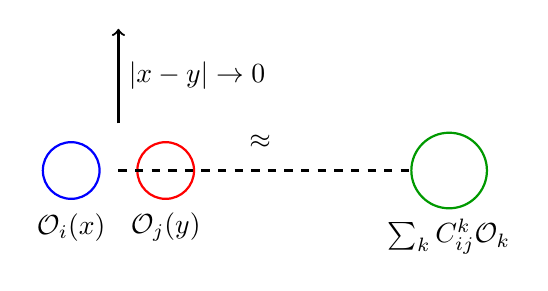
\begin{tikzpicture}[scale=1.2]
    % 两个算符靠近
    \draw[thick, blue] (0,0) circle (0.3);
    \node at (0,-0.6) {$\mathcal{O}_i(x)$};
    \draw[thick, red] (1,0) circle (0.3);
    \node at (1,-0.6) {$\mathcal{O}_j(y)$};
    \draw[thick, ->] (0.5,0.5) -- (0.5,1.5) node[midway, right] {$|x-y| \to 0$};
    % OPE 展开
    \draw[thick, green!60!black] (4,0) circle (0.4);
    \node at (4,-0.7) {$\sum_k C_{ij}^k \mathcal{O}_k$};
    \draw[thick, dashed] (0.5,0) -- (3.6,0);
    \node at (2, 0.3) {$\approx$};
\end{tikzpicture}
\caption{算符乘积展开（OPE）的示意图。当两个算符 $\mathcal{O}_i(x)$ 和 $\mathcal{O}_j(y)$ 足够接近时，它们的乘积可以展开为其他算符 $\mathcal{O}_k$ 的和。}
\label{fig:ope_diagram}
\end{figure}

\subsection{OPE 的结构}

\begin{theorem}[OPE 的共形结构]
在 CFT 中，OPE 的结构由共形对称性完全确定。对于两个标量初级算符，OPE 为：
\begin{equation}
    \mathcal{O}_i(x) \mathcal{O}_j(y) = \sum_k C_{ij}^k \frac{1}{|x-y|^{\Delta_i+\Delta_j-\Delta_k}} \left[ \mathcal{O}_k(y) + \text{后裔算符} + \cdots \right].
\end{equation}
OPE 系数 $C_{ij}^k$ 是无量纲常数，它包含了理论的非平庸信息。
\end{theorem}

\begin{remark}[OPE 的收敛性]
在 CFT 中，OPE 具有非平庸的收敛半径。当 $|x-y|$ 小于到其他算符的距离时，OPE 收敛。OPE 的收敛性告诉我们，当两个算符足够接近时，它们的行为可以用其他算符来描述。这类似于物理学中的多极展开（multipole expansion）：当距离足够远时，电荷分布可以用多极矩来描述。
\end{remark}

\subsection{OPE 系数的性质}

\begin{property}[OPE 系数的结合律]
OPE 系数 $C_{ij}^k$ 包含了理论的非平庸信息。它们满足结合律（associativity）：
\begin{equation}
    \sum_m C_{ij}^m C_{mk}^l = \sum_m C_{jk}^m C_{im}^l.
\end{equation}
结合律保证了 OPE 的一致性：无论我们以什么顺序进行 OPE，最终结果都应该相同。这类似于量子力学中的算符结合律：$(AB)C = A(BC)$。
\end{property}

\begin{property}[OPE 系数的对称性]
\begin{equation}
    C_{ij}^k = C_{ji}^k.
\end{equation}
\end{property}

\subsection{OPE 与关联函数}

\begin{theorem}[OPE 与四点函数]
OPE 系数与共形块一起决定了四点函数：
\begin{equation}
    \langle \mathcal{O}_1(x_1) \mathcal{O}_2(x_2) \mathcal{O}_3(x_3) \mathcal{O}_4(x_4) \rangle = \sum_{\mathcal{O}} C_{12\mathcal{O}} C_{34\mathcal{O}} G_{\Delta, l}(u, v).
\end{equation}
这可以理解为"通道展开"：在散射理论中，我们可以将散射振幅展开为不同通道的贡献之和（s, t, u 通道）；类似地，在 CFT 中，我们可以将四点函数展开为不同"共形通道"的贡献之和。
\end{theorem}

\subsection{共形自举}

\begin{definition}[共形自举]
OPE 的结合律对共形数据施加了很强的约束。这些约束可以用来\textbf{唯一地确定}某些 CFT 的共形数据，而不需要任何微扰计算。这种方法称为\textbf{共形自举}（conformal bootstrap）。

共形自举的基本思想是：OPE 的结合律等价于四点函数在不同通道展开的一致性条件。通过要求这些条件同时满足，可以得到共形数据的约束方程。在某些情况下，这些约束足够强，可以唯一地确定共形数据。
\end{definition}

%=============================================================================
\section{CFT 的物理意义与应用}

共形场论不仅仅是一个数学框架，它在理论物理学中有着深刻的物理意义和广泛的应用。

\subsection{CFT 与临界现象}

\begin{note}[物理动机]
CFT 最重要的物理应用之一是描述临界现象。在连续相变的临界点处，关联长度发散，系统表现出尺度不变性。此时，微观细节变得不重要，系统的临界行为可以由 CFT 描述。考虑一个铁磁体在居里温度附近的相变。当温度接近居里温度时，磁化强度的涨落变得长程相关，关联长度发散。此时，系统的临界行为不依赖于微观细节（如晶格结构），而只依赖于对称性和维度。
\end{note}

\begin{example}[临界现象的 CFT 描述]
\begin{itemize}
    \item \textbf{伊辛模型}：2 维伊辛模型的临界点由 $c = 1/2$ 的 CFT 描述
    \item \textbf{XY 模型}：2 维 XY 模型的临界点由 $c = 1$ 的 CFT 描述
    \item \textbf{海森堡模型}：2 维海森堡模型的临界点由 $c = 3/2$ 的 CFT 描述
\end{itemize}
\end{example}

\subsection{CFT 与弦理论}

\begin{note}[物理动机]
CFT 在弦理论中扮演着核心角色。弦的世界面理论是一个 2 维 CFT，这使得 CFT 成为弦理论的基础 \cite{Polchinski1998}。弦在时空中运动时，扫出一个二维曲面，称为世界面。世界面上的物理由一个 2 维量子场论描述。为了保证弦理论的自洽性（即消除共形反常），这个量子场论必须是一个 CFT。
\end{note}

\begin{example}[弦理论中的 CFT]
\begin{itemize}
    \item \textbf{玻色弦}：玻色弦的世界面理论是一个 $c = 26$ 的 CFT
    \item \textbf{超弦}：超弦的世界面理论是一个 $c = 15$ 的超对称 CFT \cite{Green1987}
    \item \textbf{弦紧致化}：弦理论的额外维度可以通过 CFT 来描述。例如，Calabi-Yau 流形上的 CFT 描述了弦的紧致化。
\end{itemize}
\end{example}

\subsection{CFT 与凝聚态物理}

\begin{example}[凝聚态物理中的 CFT]
CFT 在凝聚态物理中也有重要应用：
\begin{itemize}
    \item \textbf{量子霍尔效应}：量子霍尔效应的边缘态由手征 CFT 描述
    \item \textbf{自旋链}：1 维自旋链的低能物理由 CFT 描述
    \item \textbf{拓扑相变}：拓扑相变的临界行为由 CFT 描述
    \item \textbf{量子临界点}：量子临界点的临界行为由 CFT 描述
\end{itemize}
\end{example}

\subsection{CFT 与 AdS/CFT 对偶}

\begin{note}[CFT 在 AdS/CFT 中的角色]
CFT 是 AdS/CFT 对偶中边界理论的基础 \cite{Maldacena1997, Witten1998}。在 AdS/CFT 对偶中，边界 CFT 的物理性质对应于体空间引力理论的物理性质：
\begin{itemize}
    \item \textbf{共形对称性}：CFT 的共形对称性对应于 AdS 空间的等距对称性
    \item \textbf{算符}：CFT 的算符对应于体空间中的场
    \item \textbf{关联函数}：CFT 的关联函数对应于体空间中经典场的传播
    \item \textbf{热力学}：CFT 的热态对应于体空间中的黑洞 \cite{Witten1998b}
\end{itemize}
\end{note}

\subsection{2 维 CFT 的特殊性质}

2 维 CFT 具有特殊的性质，因为 2 维共形群是无限维的。这使得 2 维 CFT 可以被精确求解。

\begin{definition}[Virasoro 代数]
在 2 维欧几里得空间中，使用复坐标 $z = x_1 + ix_2$ 和 $\bar{z} = x_1 - ix_2$，共形变换可以分解为全纯（holomorphic）和反全纯（anti-holomorphic）两部分。

全纯共形变换的生成元为：
\begin{equation}
    L_n = -z^{n+1} \partial_z, \quad n \in \mathbb{Z}.
\end{equation}
这些生成元满足 Virasoro 代数：
\begin{equation}
    [L_m, L_n] = (m-n) L_{m+n} + \frac{c}{12} m(m^2-1) \delta_{m+n, 0},
\end{equation}
其中 $c$ 是中心荷。类似地，反全纯部分有生成元 $\bar{L}_n$ 和中心荷 $\bar{c}$。
\end{definition}

\begin{remark}
Virasoro 代数是 2 维共形代数的无限维推广。中心荷 $c$ 的出现是量子效应——在经典水平上，$c = 0$。中心荷度量了 Virasoro 代数的"中心扩张"，它在 2 维 CFT 中扮演着核心角色 \cite{Zamolodchikov1986}。
\end{remark}

\begin{proof}[Virasoro 代数中心扩展的推导]
考虑量子修正后的 Virasoro 生成元。经典对易关系为 $[L_m, L_n] = (m-n)L_{m+n}$。量子修正允许出现中心扩展项 $c_{m,n} \delta_{m+n,0}$。由 Jacobi 恒等式：
\begin{equation}
    [[L_m, L_n], L_k] + [[L_n, L_k], L_m] + [[L_k, L_m], L_n] = 0,
\end{equation}
将中心扩展项代入，得到约束：
\begin{equation}
    (m-n)c_{m+n,k} + (n-k)c_{n+k,m} + (k-m)c_{k+m,n} = 0.
\end{equation}
令 $k = -m-n$，得：
\begin{equation}
    (m-n)c_{0,-m-n} + (2n+m)c_{n,-m-n} + (-m-2n)c_{-m,-n} = 0.
\end{equation}
这要求 $c_{m,n}$ 正比于 $m(m^2-1)\delta_{m+n,0}$，因此：
\begin{equation}
    [L_m, L_n] = (m-n) L_{m+n} + \frac{c}{12} m(m^2-1) \delta_{m+n, 0}.
\end{equation}
\end{proof}

\subsection{2 维 CFT 的初级算符}

\begin{definition}[2 维初级算符]
在 2 维 CFT 中，初级算符由两个量子数标记：全纯维数 $h$ 和反全纯维数 $\bar{h}$。共形维数和自旋为：
\begin{equation}
    \Delta = h + \bar{h}, \quad s = h - \bar{h}.
\end{equation}

初级算符满足：
\begin{equation}
    L_n |\mathcal{O}\rangle = 0, \quad \bar{L}_n |\mathcal{O}\rangle = 0, \quad n > 0.
\end{equation}
\end{definition}

\subsection{2 维 CFT 的配分函数}

\begin{theorem}[环面配分函数]
2 维 CFT 的配分函数在环面（torus）上可以精确计算。环面的配分函数为：
\begin{equation}
    Z(\tau, \bar{\tau}) = \text{Tr} \left( q^{L_0 - c/24} \bar{q}^{\bar{L}_0 - \bar{c}/24} \right),
\end{equation}
其中 $q = e^{2\pi i \tau}$，$\tau$ 是环面的模参数。
\end{theorem}

\begin{property}[模不变性]
配分函数必须在模变换下不变，这施加了很强的约束。例如，$S$-变换 $\tau \to -1/\tau$ 要求：
\begin{equation}
    Z(-1/\tau, -1/\bar{\tau}) = Z(\tau, \bar{\tau}).
\end{equation}
\end{property}

%=============================================================================
\section{共形场论的例子}

\subsection{自由标量场}

\begin{example}[自由标量场 CFT]
最简单的 CFT 是自由标量场理论：
\begin{equation}
    \mathcal{L} = \frac{1}{2}(\partial_\mu \phi)^2.
\end{equation}
这个理论具有共形对称性，标量场的共形维数为 $\Delta = (d-2)/2$。自由标量场理论是可解的，所有关联函数都可以精确计算。它是 CFT 的"氢原子"：虽然简单，但包含了 CFT 的所有基本概念。

自由标量场的两点函数为：
\begin{equation}
    \langle \phi(x) \phi(y) \rangle = \frac{C_\phi}{|x-y|^{2\Delta_\phi}}, \quad \Delta_\phi = \frac{d-2}{2}.
\end{equation}
在 4 维中，$\Delta_\phi = 1$，两点函数为 $\langle \phi(x) \phi(y) \rangle = C_\phi/|x-y|^2$。
\end{example}

\subsection{Wess-Zumino-Witten 模型}

\begin{example}[WZW 模型]
2 维的 Wess-Zumino-Witten（WZW）模型是具有手征对称性的 CFT，它是弦理论和凝聚态物理中的重要模型。WZW 模型的中心荷由群的等级和维数决定：
\begin{equation}
    c = \frac{k \dim G}{k + h^\vee},
\end{equation}
其中 $k$ 是 level，$G$ 是李群，$h^\vee$ 是对偶 Coxeter 数。
\end{example}

\subsection{$\mathcal{N}=4$ 超对称杨-米尔斯理论}

\begin{definition}[$\mathcal{N}=4$ SYM]
$\mathcal{N}=4$ 超对称杨-米尔斯理论（super Yang-Mills theory）是 AdS$_5$/CFT$_4$ 对偶中的边界理论 \cite{Maldacena1997}，具有最大超对称性。

$\mathcal{N}=4$ SYM 的场内容：
\begin{itemize}
    \item 1 个规范场 $A_\mu$
    \item 4 个费米子场 $\psi_i$（$i=1,2,3,4$）
    \item 6 个标量场 $\phi_i$（$i=1,2,3,4,5,6$）
\end{itemize}
\end{definition}

\begin{property}[$\mathcal{N}=4$ SYM 的中心荷]
$\mathcal{N}=4$ SYM 的中心荷为：
\begin{equation}
    c = \frac{N^2 - 1}{4} \approx \frac{N^2}{4}.
\end{equation}
在大 $N$ 极限下，$c$ 很大，对应于经典的引力理论。
\end{property}

%=============================================================================
\section{共形场论与 AdS/CFT}

在 AdS/CFT 对偶中，边界理论是一个共形场论。共形对称性在对偶中起着核心作用 \cite{Maldacena1997}：
\begin{itemize}
    \item AdS$_{d+1}$ 空间的等距群 $SO(2,d)$ 等于 $d$ 维 CFT 的共形群
    \item CFT 的共形维数对应于 AdS 中场的质量：$\Delta(\Delta-d) = m^2 L^2$ \cite{Gubser1998}
    \item CFT 的中心荷对应于 AdS 的引力常数：$c \sim L^{d-1}/G_N$
    \item CFT 的 OPE 系数对应于 AdS 中的耦合常数
\end{itemize}

\begin{note}[对称性起源]
在 AdS/CFT 对偶中，CFT 的共形对称性自然地从 AdS 的几何对称性中产生。AdS 空间的等距变换对应于 CFT 的共形变换。这解释了为什么 AdS/CFT 对偶中的边界理论必须是一个共形场论。
\end{note}

\subsection{AdS/CFT 中的算符-场对应}

\begin{theorem}[算符-场对应]
在 AdS/CFT 中，CFT 的每个算符都对应于体空间中的一个场 \cite{Gubser1998, Witten1998}：
\begin{center}
\begin{tabular}{|c|c|c|}
\hline
\textbf{CFT 算符} & \textbf{AdS 场} & \textbf{共形维数} \\
\hline
标量算符 $\mathcal{O}$ & 标量场 $\phi$ & $\Delta(\Delta-d) = m^2 L^2$ \\
守恒流 $J_\mu$ & 规范场 $A_\mu$ & $\Delta = d-1$ \\
应力张量 $T_{\mu\nu}$ & 度规扰动 $h_{\mu\nu}$ & $\Delta = d$ \\
\hline
\end{tabular}
\end{center}
\end{theorem}

\subsection{中心荷与引力常数}

\begin{theorem}[中心荷与引力常数的关系]
CFT 的中心荷 $c$ 与体空间的引力常数相关。在 4 维中：
\begin{equation}
    c = \frac{L^3}{8\pi G_N^{(5)}} = \frac{N^2}{4}.
\end{equation}
这个关系表明，当 $N$ 很大时，$c$ 也很大，对应于经典引力。这正是 AdS/CFT 对偶在大 $N$ 极限下成立的原因 \cite{Maldacena1997}。
\end{theorem}

\begin{remark}[大 $N$ 极限]
在大 $N$ 极限下，CFT 的中心荷 $c \sim N^2$ 很大，对应于经典的引力理论。当 $N$ 有限时，量子修正变得重要，对应于弦理论的修正 \cite{Aharony1999}。
\end{remark}

%=============================================================================
\section{小结}

在本节中，我们介绍了共形场论的基本概念：
\begin{itemize}
    \item 共形变换是保持角度不变的坐标变换，共形群是 $SO(2,d)$
    \item 共形代数由平移、旋转、标度变换和特殊共形变换生成
    \item 共形维数描述算符在标度变换下的行为，初级算符是共形群的最低权态
    \item 共形对称性对关联函数施加很强的约束：一点函数为零，两点和三点函数完全确定
    \item 共形 Ward 恒等式将守恒律与关联函数的对称性联系起来
    \item 共形异常反映了经典对称性在量子水平上的破缺，$a$-定理描述了 RG 流的不可逆性 \cite{Komargodski2011}
    \item 算符乘积展开是 CFT 中最重要的工具，共形自举可以唯一确定某些 CFT 的共形数据
    \item 2 维 CFT 具有无限维的 Virasoro 代数，可以被精确求解 \cite{Zamolodchikov1986}
    \item CFT 是 AdS/CFT 对偶中边界理论的基础 \cite{Maldacena1997}
\end{itemize}

\begin{note}[进一步阅读]
关于共形场论的更多细节，读者可以参考 \cite{Natsuume2014, Ammon2015, Aharony1999}。关于共形自举的最新进展，可以参考相关综述文献。关于 2 维 CFT 的精确求解方法，Zamolodchikov 的经典论文 \cite{Zamolodchikov1986} 是必读文献。
\end{note}

%=============================================================================
